\documentclass[11pt]{article}

\usepackage{fullpage}
\usepackage{amsfonts}
\usepackage{graphicx}

\graphicspath{ {img/} }

\def\eq1{y=\frac{x}{3x^2+x+1}}
\def\labelaxes{sedang membuat fungsi pada sebuah dokumen \LaTeX}

\begin{document}
	
	\begin{center}
	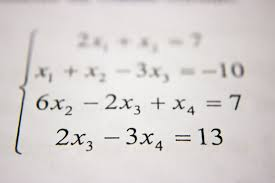
\includegraphics[scale=0.5]{1.jpg}
	
	image di simpan dengan format .png, .jpg, .gif, atau .pdf files.
	\end{center}
	
	The set of Natural number is denoted by $\mathbb{N}$.
	
	The set of Integral is denoted by $\mathbb{Z}$.
	
	The set of Real number is denoted by $\mathbb{R}$.
	
	Graph $\eq1$. \labelaxes
	
	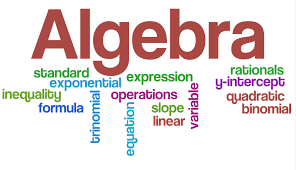
\includegraphics[width=5in]{2.png}
	
	Identify the asymptotes for the graph of $\eq1$.
	
\end{document}